\chapter{Теоретическое введение}
\section{Процессы реального времени}
Абстрактный процесс в системе определяется как последовательность $ \langle P_0,P_1,...\rangle $   состояний системы, а процесс реального времени – как последовательность упорядоченных пар $ \langle P_i,t_i \rangle, i\in N_0 $\footnote{$ N_0 \cong \{0,1,2,\dots\}$} представленных состояниями системы и временами переходов системы в эти состояния, причем времена в последовательности строго упорядочены по возрастанию. 
Далее мы будем рассматривать только процессы реального времени. 
В общем случае для недетерминированных систем процессы представлены конечными или бесконечными путями из корня дерева процессов. 
Корень дерева процессов представляет собой пару $ \langle P(t_0),0 \rangle $ , где $ P_0 $  – начальное состояние всех заданных этим деревом процессов в момент времени  $ t_0 = 0 $. 
В понятии процесса используется понятие времени, как абстрактного, представленного номерами в образующей процесс последовательности, так и реального, представленного элементами числовой шкалы времени, которая представлена линейно упорядоченным множеством моментов времени и, желательно: 
\begin{itemize}
	\item включает минимальное и максимальное значения, 
	\item имеет разрешимые предикаты сравнения ($ <,\leq,=,\geq, > $),
	\item является плотной, в которой для любых различных моментов времени $ t^{'} $  и $ t^{''} $  , таких, что $ t^{'}<t^{''} $ , существует момент времени $ t $ , такой, что  $ t^{'}<t $  и $ t<t^{''} $ .
\end{itemize}

Не ограничивая общности, будем в качестве удовлетворяющей этим требованиям шкалы времени рассматривать множество $ Q = Q \cup \{\omega\} $, где $ Q=Q_+\cup{0} $ ,$ Q_+ $~--- множество положительных рациональных чисел, $ 0 $ --- минимальное значение:$ (\forall t \in Q_+) (0<t) $ , $ \omega $--- несобственное значение, время, неограниченно отдаленное в будущем: $ (\forall t \in Q) (t<\omega) $. 
Сохраняя основные свойства арифметических операций, доопределим естественным образом для элементов множества $ Q $ указанные отношения $ <,\leq,=,\geq, > $ и арифметические операции сложения, вычитания, умножения и деления, за исключением некоторых случаев: $ \omega/\omega $ , $ 0/0 $ , $ 0*\omega $  и вычитания из меньшего значения большего. 
Заметим, что положительные рациональные числа представляются упорядоченными парами положительных натуральных чисел, в общем случае неоднозначно. Каноническое представление предполагает, что эти числа являются взаимно-простыми. Через $ \tau $   будем далее обозначать текущее время в системе, через $ t\in Q $  --- произвольный момент времени.  

\section{Понятие эпизода}
В основе предлагаемых далее определений мы используем понятие эпизода. 
Эпизоды задаются их типами и двумя моментами времени: начала и завершения (более точно определено ниже). 
Неформально, эпизоды~--- некие сущности (объекты, свойства и т.п.) на интервалах рассматриваемой шкалы времени. 
Интервал~--- упорядоченная пара $ \langle t^{'},t^{''}\rangle $ моментов времени, такая, что  $ t^{'}<t^{''} $. 
Состояние системы в любой момент времени $ t $ определяется как неупорядоченный набор (комплект, конечное мультимножество) не завершившихся к этому времени эпизодов.

Пусть $ p\equiv \langle e,\theta \rangle $~--- эпизод. 
Первый компонент представляет тип эпизода из не более чем счетного множества  $ E $  типов эпизодов в рассматриваемой системе. 
Важную роль в описании частных случаев определения процессов в системах играет структуризация множества типов эпизодов. 
Разбиение типа на два компонента практически не ограничивает общности: $ E \equiv E_B \times E_D $. 
Первый компонент типа определяет возможные события в системе, приводящие к изменению ее состояния, а второй~--- наполняет их конкретным содержанием. 
Для всех  $ \langle e_B,e_D \rangle \in E $  полагаем, что $ e_B $~--- структурный атрибут эпизода, $ e_D $~--- его информационный атрибут. 
Практически полезной является и дальнейшая детализация структурного атрибута: полагаем, что $ e_B \equiv \langle e_B^{'}, e_B^{''} \rangle $ , где $ e_B^{'} $~--- один из группирующих эпизоды контейнеров, к которому <<относится>> (или, иначе говоря, в котором <<находится>> эпизод), а $ e_B^{''} $~--- сорт (или тег) эпизода, уточняющий средства оперирования с информационными атрибутами (аналог понятия типа или класса информационных объектов в языках программирования). 
В частном случае, сорт эпизода может однозначно определяться его контейнером. 
В свою очередь, сорт эпизода определяет множество возможных значений его информационного атрибута. 
Предполагается, что множество значений информационного атрибута любого сорта содержит неопределенное значение  $ \perp $.

Второй компонент эпизода $ \theta \equiv \langle t^{'} t^{''} \rangle \in Q \times Q $, $ t^{'}<t^{''} $ задает временные характеристики конкретного эпизода: $ t^{'}\in Q $  определяет начало эпизода на шкале времени; $ t^{''}\in Q $ , если эпизод завершен ($ \tau \geq \tablename^{''} $), то это ~--- конец эпизода, иначе эпизод полагается незавершенным, и $ \delta \cong t^{''}-t^{'} > 0 $ понимается как предельно возможная длительность незавершенного эпизода (если $ t^{''}=\omega $ , то возможная длительность эпизода сверху не ограничена). 

\section{События}

Изменение состояний системы в автоматной модели определяется как ее текущим состоянием, так и действующим интерфейсом, который устанавливает взаимосвязь эпизодов и, в общем случае, сам тоже может изменяться при переходах системы к новым состояниям. В каждый момент времени действующий интерфейс определяет для текущего состояния системы возможность событий, в результате которых могут измениться и состояние системы, и действующий интерфейс. 
Событие~--- переход системы в новое состояние, который характеризуется моментом времени этого перехода и определяется временем ближайшего предшествующего события, текущим состоянием системы и действующим интерфейсом эпизодов. 
Первопричинами основных событий являются: 
\begin{enumerate}
	\item появление в состоянии системы наборов (комплектов) эпизодов, необходимые требования к которым и определяет действующий интерфейс, 
	\item  а в рассматриваемых далее динамических системах~--- подключение к системе определенным образом модифицированных копий подсистем. 
\end{enumerate}
Изменение состояния системы возможно также в связи с достижением максимально возможного времени окончания некоторого эпизода, в этом случае такой эпизод исключается из состояния системы и не может влиять на последующие события. 
Информационный атрибут такого завершенного эпизода полагается равным $ \perp $.

\section{Интерфейс системы}
Согласно нашему первоначальному замыслу, основные объекты в определении понятия системы~--- состояние системы, интерфейс, элемент интерфейса – должны были быть определены как неупорядоченные наборы, соответственно, незавершенных эпизодов, элементов интерфейса и требований к структурным атрибутам эпизодов, необходимых для срабатывания элементов интерфейса, составляющих события в системе, приводящие к изменению ее состояния. 
Однако, вследствие этого появляется значительная неопределенность в поведении системы, выражающаяся в чрезмерном разрастании дерева процессов. Для предотвращения этого мы отказались от концепции неупорядоченности, что позволило ввести в описание систем разного рода приоритеты, устраняющие во многом недетерминированность поведения систем. 
Фактически, неоднозначность появляется только вследствие маловероятного случайного совпадения времени готовности к срабатывания структурно не связанных элементов интерфейса и по причине сознательного отказа от учета информационных атрибутов эпизодов в формировании событий в системе, оставив только их влияние на результат~--- возможные изменения состояния системы.

В дальнейшем будем различать два варианта систем: с последовательным и параллельным интерфейсом.

В общем случае интерфейс рассматривается как упорядоченное множество элементов интерфейса, причем требование упорядоченности используется, во-первых, для приоритетного применения элементов интерфейса для систем с последовательным интерфейсом, во-вторых, для приоритетного распределения эпизодов состояния системы при одновременном срабатывании комплекта элементов интерфейса для систем с параллельным интерфейсом.
Каждый отдельный элемент интерфейса определяет кортеж требований к элементам соответствующего ему набора эпизодов, а именно, к их контейнерам и (или) сортам, а также к временам их появления (к началам эпизодов) по отношению к минимально возможному моменту предполагаемого их совместного срабатывания – в виде так называемой <<выдержки>> эпизодов с областью значений $ Q_+ $ . 
Если из элементов текущего состояния системы можно сформировать соответствующий элементу интерфейса кортеж эпизодов, то будем говорить, что он готов к срабатыванию в рассматриваемый момент времени. 
Ограничить разнообразие удовлетворяющих этим требованиям комплектов эпизодов можно дополнительно заданием для конкретного элемента интерфейса одной из двух основных дисциплин выбора эпизодов из текущего состояния системы: FIFO – предпочтение отдается <<старым>> эпизодам (с более ранним началом) или LIFO  предпочтение отдается <<молодым>> эпизодам (с более поздним началом). 
В простейшем случае элементы действующего в текущий момент времени интерфейса могут быть заданы путем их непосредственного перечисления, разумеется, если их конечное число. 
В более общем случае, который в этой статье не рассматривается, интерфейс задается в форме некоторой схемы – выражений формального языка, содержащих, возможно, свободные вхождения переменных с известными областями значений, причем возможными значениями этих выражений являются отдельные элементы интерфейса, а само множество значений является рекурсивно-перечислимым (и, в общем случае, может быть бесконечным). 

Для систем с последовательным интерфейсом отдельные его элементы анализируются на возможность срабатывания в порядке их перечисления, вплоть до первого готового к срабатыванию в ближайший момент времени по отношению к времени предыдущего события. Очевидно, что в один и тот же момент времени может произойти последовательное срабатывание нескольких элементов интерфейса в порядке их перечисления.

Для систем с параллельным интерфейсом отдельные элементы интерфейса определяют только возможность событий в системе. В системе выделяются готовые к одновременному срабатыванию в некоторый момент времени подкомплекты эпизодов текущего состояния системы при условии ненаступления до этого других событий. Поэтому переход к новому состоянию системы, как и для систем с последовательным интерфейсом, может стать реальным только для возможных событий с минимальным ожидаемым временем. Если это время окажется больше максимально возможного времени окончания хотя бы одного из выбранных эпизодов, то для определения готовности всё следует повторить для состояния, в котором удалены такие эпизоды. Если требуемых комплектов эпизодов нет, то процесс завершается; в противном случае рассматривается готовность к одновременному срабатыванию всевозможных комплектов указанных комплектов эпизодов для отдельных элементов параллельного интерфейса. Хотя при этом рассматривается возможность выделения в состоянии системы комплектов эпизодов на основе <<смешивания>> упорядоченных по времени выдержки подкортежей требований к различным значениям структурных атрибутов эпизодов, необходимых для срабатывания элементов интерфейса, однако, сам выбор конкретных эпизодов и сама возможность такого выбора с полученным на первом этапе минимально возможным временем срабатывания могут оказаться иными даже при условии сохранения дисциплины выбора, индивидуально заданной для каждого элемента интерфейса. Полагаем, что фактически смогут реализоваться только максимальные из этих готовых к совместному срабатыванию комплектов элементов интерфейса. Реализуемый таким образом принцип максимально возможного параллелизма в поведении системы позволяет исключить из рассмотрения события с одним и тем же временем. Если таких максимальных суммарных комплектов более одного, то поведение системы становится недетерминированным, и, как было сказано ранее, оно формализуется в виде дерева процессов: происходит его ветвление, вершина текущего состояния системы будет иметь несколько потомков, по одному для каждого указанного выше случая. Каждый из вариантов определяет и свой результат соответствующего события, т.е. изменения состояния системы и действующего интерфейса. 

\section{Результат события}
Перейдем к краткому рассмотрению результата события – к изменениям состояния системы, а для динамических систем и действующего интерфейса. 

Пусть процесс не обрывается и $ t_{i+1} $  – время очередного события. 
Во-первых, из состояния $ P_i $ уже исключены эпизоды, время максимально возможного окончания которых меньше $ t_{i+1} $. 
Участвующие в событии эпизоды также исключаются из состояния системы. 
Каждый из участвовавших в событии элемент интерфейса порождает, с учетом его кратности вхождения в реализованный в событии комплект элементов интерфейса, комплект новых эпизодов, добавляемых к текущему состоянию системы (после указанных выше удалений эпизодов). 
Для каждого нового эпизода задаются полностью (и контейнеры, и сорта) структурные атрибуты, <<задержка>> (число из $ Q $ ), результат сложения которого с  $ t_{i+1} $  дает начало этого эпизода, и еще одно число из $ Q $ . 
Если оно равно нулю, то длительность нового эпизода не ограничена сверху (параметр <<конец эпизода>> получает значение $ \omega $ ), в противном случае он задает положительную длительность эпизода, а значение параметра <<конец эпизода>> получается сложением длительности с началом эпизода. 
Все это, в сочетании с требованием задания положительных значений для выдержек, гарантирует отсутствие готовности к срабатыванию в момент времени $ t_{i+1} $ новых, появившихся в результате рассматриваемого события, эпизодов в состоянии системы. 
В общем случае все характеристики новых эпизодов определяются как значения заданных для каждого элемента интерфейса функций из функционального базиса системы, согласованных по сортам аргументов с сортами входных эпизодов элемента интерфейса. 
Значениями аргументов этих функций выступают значения информационных атрибутов выделенных в состоянии системы $ P_i $ участвующих в событии эпизодов для рассматриваемого элемента интерфейса. 
Именно с целью установления соответствия аргументов и их значений перечисление требований к эпизодам уже в элементе интерфейса осуществляется в некотором порядке, т.е. в форме кортежа. 
В частном случае, структурные атрибуты (контейнеры, сорта) и максимально возможные времена окончаний новых эпизодов задаются непосредственно в элементе интерфейса, если всем сортам эпизодов сопоставлены одноэлементные множества возможных значений информационных атрибутов. 

Описанные события не приводят к изменению интерфейса системы, множество используемых контейнеров ограничено множеством контейнеров, фигурирующих в начальном состоянии системы и ее интерфейсе. 
Такие системы будем называть статическими. 
Для описания поведения динамических систем, интерфейс которых может изменяться во времени, а множества используемых контейнеров неограниченно расширяться, нужны совсем иные пути формализации для реализации этих возможностей. 
Не претендуя на общность, мы предлагаем дополнительно ввести в качестве элементов интерфейсов динамических систем так называемые нетерминальные элементы, в то время как рассмотренные ранее будем называть терминальными элементами интерфейсов. 

Если для терминальных элементов интерфейса эффект выражается в создании новых эпизодов и сохранении действующего интерфейса, то в результате срабатывания нетерминального элемента интерфейса происходят структурные изменения: могут появиться новые элементы интерфейса, могут появиться не только новые эпизоды в состоянии системы, но и новые контейнеры. 
Вопрос же об удалении из рассмотрения некоторых контейнеров и элементов интерфейса должен решаться подобно тому, как решается проблема <<сборки мусора>> для памяти типа <<куча>>.

Динамическая система представлена в виде конечного множества именованных подсистем, каждая из которых задана тройкой~--- начальным состоянием, начальным интерфейсом и упорядоченным конечным подмножеством контейнеров подсистемы, элементы которого будем называть контактами подсистемы. 
Контейнеры подсистемы, не вошедшие в число контактов, при срабатывании нетерминального элемента интерфейса и подключении к системе этой подсистемы будут представлять новые контейнеры, отличные от всех ранее используемых в системе. 
Механизм порождения новых контейнеров аналогичен процессу выделения новых ячеек в памяти типа <<куча>> и, в какой-то мере, операции замены связанной переменной в формальных системах с операторами, связывающих вхождения операторной переменной в терм, к которому применяется оператор (например в $ \lambda $-исчислении). 
Вершина дерева процессов (начальное состояние системы) представлена начальным состоянием выделенной базовой подсистемы (аксиомы). 
Предполагается возможность в дальнейшем подключений к системе любых подсистем, в том числе и подсистемы-аксиомы. 
Множество имен всех подсистем образуют особый сорт $ D $ значений информационных атрибутов эпизодов.

В текущем интерфейсе всякий нетерминальный элемент представлен следующей информацией: 
\begin{enumerate}
	\item контейнером, наличие в котором эпизода сорта $ D $   может привести к срабатыванию этого нетерминального элемента, 
	\item  выдержкой, играющей ту же роль, что и выдержки эпизодов в терминальных элементах интерфейса, 
	\item  кортежем контейнеров текущего состояния системы, элементы которого будем называть контактами рассматриваемого нетерминального элемента текущего интерфейса (заметим, что один и тот же контейнер может входить неоднократно в указанный кортеж), 
	\item  функцией, аргументом которой является имя подсистемы, а значением – задержка подключения соответствующей подсистемы из множества $ Q $ .
\end{enumerate}  

Условием возможного срабатывания нетерминального элемента интерфейса в момент времени $ t_{i+1} = t_i + \delta $ , где $ \delta $~--- указанная для этого элемента <<выдержка>>, является просто наличие в состоянии системы соответствующего эпизода сорта $ D $ в указанном контейнере. 
В результате срабатывания нетерминального элемента интерфейса происходит подключение к системе некоторой подсистемы, имя которой определяется информационным атрибутом эпизодов, что приводит к изменениям основных компонентов состояния системы, помимо тех, которые вносятся в результате возможного одновременного срабатывания терминальных элементов интерфейса. 
Одна из основных проблем определения процедуры подключения подсистемы состоит в том, чтобы она исключала возможность в момент времени подключения срабатывания новых элементов обновленного интерфейса. 
Кроме того, при одновременном срабатывании нескольких нетерминальных элементов результат подключения нескольких подсистем не должен зависеть от порядка их реализации.

\subsection{Подключение подсистемы}
Опишем вначале способ подключения к системе некоторой одной подсистемы.

Как было сказано ранее, для выполнения подключений каждая подсистема, помимо ее начального состояния и начального интерфейса, содержит контактную информацию для ее подключений, и, в свою очередь, всякий нетерминальный элемент действующего интерфейса системы также содержит свою контактную информацию. 
Контактная информация позволяет установить связь между контейнерами основной системы и контейнерами подключаемой подсистемы путем замены контейнеров в подключаемой системе на соответствующие (согласно порядкам перечисления контактов) контейнеры основной системы; 
именно для того, чтобы при подключении не возникла возможность <<ложных>>, не реализованных к моменту подключения срабатываний элементов действующего интерфейса системы, соответствующая контактная информация в основной системе задается в форме кортежа используемых в ней контейнеров, а в подключаемой подсистеме --- в форме упорядоченного подмножества используемых в ней контейнеров, причем для остальных контейнеров подключаемой подсистемы производится их замена на новые контейнеры, не используемые ранее в основной системе. 
При подключении подсистемы начала всех эпизодов во всех ее контейнерах формируются путем сложений их начал и, соответственно, концов, заданных в начальном состоянии подключаемой подсистемы, времени события, включающего срабатывание рассматриваемого нетерминального элемента основной системы, и задержки подключения соответствующей подсистемы при срабатывании конкретного нетерминального элемента интерфейса системы. 
Так как новый интерфейс системы в результате срабатывания нетерминального элемента пополняется элементами интерфейса подключаемой подсистемы, то указанное изменение временных параметров подключаемых к состоянию системы эпизодов подсистемы не может привести к готовности в тот же момент времени к срабатыванию как <<старых>>, так и <<новых>> элементов интерфейса. 
Очевидно, что, так как интерфейс подключаемых подсистем может тоже содержать нетерминальные элементы, то в системе может неограниченно увеличиваться количество используемых контейнеров и элементов интерфейса, а описанная далее <<сборка мусора>> в системе может приводить к удалению <<лишних>> эпизодов, контейнеров и элементов интерфейса.

В общем случае, событие, приводящее к изменению состояния системы в момент времени $ t_{i+1} $ , может включать одновременное срабатывание не только нескольких терминальных элементов интерфейса, но и нескольких его нетерминальных элементов. 
Подключение одной подсистемы предполагает следующую последовательность шагов:
\begin{itemize}
	\item создание рабочих копий начального состояния и начального интерфейса выбранной для подключения подсистемы (далее под состоянием и интерфейсом подключаемой подсистемы будем понимать эти копии); 
	изменение в состоянии и интерфейсе подключаемой подсистемы временных параметров эпизодов так, как было описано выше;
	\item замена различных контейнеров в состоянии и интерфейсе подключаемой подсистемы на различные новые контейнеры, не используемые ни в текущем состоянии и интерфейсе системы, ни в начальном состоянии и интерфейсе подключаемой подсистемы;
	\item замена всех контейнеров в состоянии и интерфейсе подключаемой подсистемы, входящих в число ее контактов, на соответствующие им по порядку контейнеры в кортеже контактов рассматриваемого нетерминального элемента интерфейса (если в последнем <<хватает>> контактов);
	\item к состоянию системы присоединяется состояние подключаемой подсистемы (путем сложения представляющих их комплектов), а к интерфейсу систем добавляется интерфейс подключаемой подсистемы (путем конкатенации представляющих их кортежей).
\end{itemize}

\section{Вывод}
В своей работе мы предполагаем и наличие принципиальных отличий даже базовых понятий: 
\begin{itemize}
	\item отказ от переходов с пустым комплектом входных позиций: в этом отношении мы обобщаем принцип <<отсутствие необходимых ресурсов (фишек) не может служить основанием каких-либо событий (переходов)>>. Это требование, не являясь принципиальным при рассмотрении поведения системы в абстрактном времени, для реального времени является принципиальным;
	\item введение линейных порядков на множествах входных и выходных позиций переходов уже используются во многих обобщениях формализма сетей Петри, и, как следствие, замена понятий <<комплект входных (выходных) позиций перехода>> на понятия <<кортеж входных (выходных) эпизодов для элемента интерфейса>>. В  нашем формализме это необходимо для описания роли информационных атрибутов эпизодов;
	\item срабатывание переходов (элементов интерфейса) управляется не только наличием фишек во входных позициях (контейнерах), а и их окраской (сортами эпизодов);
	\item изменение состояний происходят в реальном, а не в абстрактом (модельном) времени, что позволяет строить более адекватные модели поведения реальных систем;
	\item в нашем подходе всегда реализуется максимально возможный параллелизм срабатывания элементов интерфейса (в базовой модели сетей Петри не допускается одновременное срабатывание нескольких переходов, а моделирование этого делает сеть неоправданно громоздкой). Этот подход позволяет в системе реального времени избавиться от возможности нескольких событий с одинаковым временем;
	\item наконец, главное: сами рассматриваемые нами системы являются динамическими, могут структурно меняться во времени и иметь при функционировании априори не ограниченную сложность.
\end{itemize}

Изменением терминологии мы хотим подчеркнуть следующую основные цели нашей публикации: описание проходящих в реальном времени параллельных вычислительных процессов в динамических системах с априори не ограниченной сложностью.

\chapter{Требования к реализации}
\section{Постановка задачи программного комплекса}

Необходимо построить программный комплекс, реализующий описанный формализм параллельных вычислительных процессов.

Общее решение должно состоять из следующих компонент:
\begin{itemize}
	\item Язык описания системы.
	\item Управляющая программа (аналог виртуальной машины).
	\item Модуль визуализации.
\end{itemize}


\subsection{Язык описания системы}
Задача построения динамических систем всё чаще возникает в современной разработке. 
Чаще всего фундаментом такой разработки является язык общего назначения, применимый к широкому спектру областей и не учитывающий осбенности конкретной сферы знаний.
Этот инструмент, вместе с гибкостью, приносит и массу проблем, связанных с резко возрастающей сложностью реализации и сопровождения системы в процессе роста программного комплекса.
Алтернативой могут служить предметно-ориентированные языки.

Предметно-ориентированный язык (англ. domain-specific language, DSL)~--- язык программирования, специализированный для конкретной области применения.
Такие языки часто встречаются в вычислениях:
\begin{itemize}
	\item CSS (англ. Cascading Style Sheets)~--- формальный язык описания внешнего вида документа, написанного с использованием языка разметки.
	\item Регулярные выражения (англ. regular expressions)~--- формальный язык поиска и осуществления манипуляций с подстроками в тексте, основанный на использовании метасимволов (символов-джокеров, англ. wildcard characters).
	\item Различные средства автоматизации сборки и тестирования программ: make, rake, ant, gradle.
	\item SQL (англ. Structured Query Language)~--- язык программирования, применяемый для создания, модификации и управления данными в реляционной базе данных, управляемой соответствующей системой управления базами данных.
	\item и т.д.
\end{itemize}
Все они позволяют разработчику описывать систему, используя термины предметной области.

В нашем случае такой язык должен включать сведения о структуре системы и её подсистем, о возможных типах данных, а также об исполняемых процедурах. 
Последнее возможно реализовать, например, за счёт ссылки на файл подпрограммы, или инъекцией сторонних языков.

DSL могут быть как текстовыми, так и графическими. 
Для графических языков требуется дополнительное программное обеспечение, позволяющее редактировать графическое представление.

Предполагается создание как текстового языка, так и графического расширения для него, позволяющего манипулировать структурными данными.

Для исполнения программы DSL должен быть преобразован представление задачи на языке управляющей программы.
\subsection{Управляющая программа}

Управляющая программа~--- реализация на языке программирования общего назначения процесса исполнения описанной вычислительной системы.
Управляемая пользователем, она должна производить вычисления и обеспечивать доступ к информации о процессе вычисления и состоянии системы.
Правила и алгоритмы исполнения описаны в первой главе.
В результате работы такой программы должен быть осуществлён вывод результата, а также, при необходимости, запрошенные метрики процесса: время, ускорение и другие.


\subsection{Модуль визуализации}
Проектирование систем параллельных вычислений~--- сложная и трудоёмкая задача, требующая от исполнителя глубокого понимания структуры и процессов, возможных и происходящих в сети. 
Облегчить её может визуализация структуры и состояния вычислительной сети.

Модуль визуализации~--- клиентская программа, позволяющая следить за ходом исполнения вычислительной задачи, предоставляющая необходимые метрики, а также возможность влияния на процесс вычислений.

Таким образом модуль визуализации должен отображать:
\begin{itemize}
	\item текущий интерфейс вычислительной сети,
	\item кнопки для управления процессом вычисления,
	\item результаты вычислений,
	\item значения, графики и сводные таблицы метрик выполнения вычислений для оценки реализации.
\end{itemize}

\chapter{Выбор инструментов} 

\section{Язык программирования}
Выбор языка программирования --- важное решение, влияющее на простоту написания и поддержки системы, возможности масштабирования, а также ограничения эксплуатации программы.

Выделим следующие важные характеристики языка:
\begin{enumerate}
%	\item Поддержка функциональной парадигмы программирования;
	\item Возможность написания кроссплатформенных программ. Кроссплатформенность --- способность ПО работать более чем на одной аппаратной платформе и операционной системе.
	\item Безопасность ~--- набор характеристик, определяющих то, насколько рано инфраструктура работы с программой на конкретном языке может определить ошибку. 
	\begin{enumerate}
		\item Статическая типизация — приём, широко используемый в языках программирования, при котором переменная, параметр подпрограммы, возвращаемое значение функции связывается с типом в момент объявления и тип не может быть изменён позже (перемнная или параметр будут принимать, а функция — возвращать значения только этого типа).
		\item Валидация во время компиляции.
	\end{enumerate}
	\item Высокий уровень языка.
	\item Поддержка рефлексии. Рефлексия (англ. reflection)~--- процесс, во время которого программа может отслеживать и модифицировать собственную структуру и поведение во время выполнения.
	\item Совместимость с другими языками программирования. 
	\item Краткость. Выражается возможности автоматической генерации кода, использования $ \lambda $-нотации для описания функции, вывод типов данных.
	\item Возможность описания предметно-ориентированных языков. Не обязательное, но желательное требование.
\end{enumerate}

\subsection{С++}
C++~---компилируемый, статически типизированный язык программирования общего назначения.

Поддерживает такие парадигмы программирования, как процедурное программирование, объектно-ориентированное программирование, обобщённое программирование. 
Язык имеет богатую стандартную библиотеку, которая включает в себя распространённые контейнеры и алгоритмы, ввод-вывод, регулярные выражения, поддержку многопоточности и другие возможности. 
C++ сочетает свойства как высокоуровневых, так и низкоуровневых языков. 
В сравнении с его предшественником — языком C, — наибольшее внимание уделено поддержке объектно-ориентированного и обобщённого программирования.

Для обеспечения кроссплатформенности программы необходимо использовать кроссплатформенные фреймворки, которых, к слову, становится всё больше и больше.
Программист C++ вынужден контролировать выделение и освобождение памяти, что является отрицательным для фактора безопасности, т.к. вносит значительную вероятность ошибки, источник которой отследить крайне сложно.

Язык не предоставляет поддержку рефлексии, однако существует расширения языка Qt, позволяющего осуществлять доступ к специально описанным объектам системы, наследникам QObject.

C++ сочетает в себе свойства языков высокого и низкого уровней.

Код на C++ достаточно громоздкий, а возможности кодогенерации ограничены использованием макросов - шаблонов кода, определёнными для препроцессора. 
Однако язык позволяет использовать $ \lambda $-выражения для описания функций.

\subsection{Java}

Java~--- сильно типизированный объектно-ориентированный язык программирования, разработанный компанией Sun Microsystems (в последующем приобретённой компанией Oracle). 
Приложения Java обычно транслируются в специальный байт-код, поэтому они могут работать на любой компьютерной архитектуре, с помощью виртуальной Java-машины.
Также возможна ahead-of-time компиляция в машинный код частей программ или программ целиком.

Язык достаточно безопасен, компилятор осуществляет валидацию кода и способен детектировать большую часть ошибок, однако в нём отсутствуют некоторые выразительные возможности, связанные с типами. 
Основной проблемой считается null-уязвимость типа. 
Проблема заключается в отсутствии возможности указать компилятору, может ли переменная принимать значение null, и при запрете, выдавать ошибку при некорректном присвоении значения.

Ещё одним плюсом для безопасности использования является модель памяти Java, в которой отсутствует необходимость явно выделять/освобождать память объектов. 
Java содержит библиотеку поддержки рефлексии, совместима со статическими библиотеками, написанными на C, а также поддерживает $ \lambda $-нотацию.

Программа на языке Java не будет сильно отличаться по размеру от аналогичной, написанной на C++. 
Однако язык позволяет писать расширения компилятора, генерирующие байт-код. 
Существует множество библиотек, позволяющий писать исходный код более кратко, а также дополняющих язык различными проверками при компиляции.

Java не позволяет описать DSL.

\subsection{Kotlin}

Kotlin (Котлин)~--- статически типизированный язык программирования высокого уровня, работающий на JVM (Java Virtual Machine) и разрабатываемый компанией JetBrains. 
Компилируется также в JavaScript и на другие платформы через инфраструктуру LLVM. 
Язык назван в честь острова Котлин в Финском заливе, на котором расположен город Кронштадт.
Авторы ставили целью создать язык более лаконичный и типобезопасный, чем Java. 

Язык Kotlin один из самых безопасных на сегодняшний день.
Помимо статической типизации, он также решает проблемму null-уязвимости типа данных.
На уровне языка поддерживается много шаблонов проектирования.
В т.ч. шаблоны <<одиночка>>, <<builder>>, DSL.
Также язык очень ёмкий и предоставляет множество удобных операторов.
Поддерживает $ \lambda $-выражения.

Язык совместим с Java.
Возможно построение мультиплатформенных приложений, когда одна и та же модель данных используется для серверной и клиентской частей приложения на базе C++, Java или JavaScript.

\subsection{Итог}

Учитывая обозначенные выше критерии, можно сделать вывод, что язык Kotlin подходит для реализации управляющей программы лучше всего.
\begin{tabular}{|c|c|c|c|}
			\hline
			Язык & С++ & Java & Kotlin \\ \hline
			Кроссплатформенный & +- & + & + \\ \hline
			Статическая типизация & + & + & + \\ \hline
			\begin{tabular}{@{}c@{}}Валидация при \\ компиляции\end{tabular}
			 & +- & +- & + \\ \hline
			Уровень & высокий + низкий & высокий &  высокий \\ \hline
			Рефлексия & - & + & + \\ \hline
			 \begin{tabular}{@{}c@{}}Совместимость с\\ другими языками\end{tabular}  & Assembler & C++, Kotlin & 			\begin{tabular}{@{}c@{}}Java, C++,\\ JavaScript \end{tabular}\\ \hline
			Краткость & 
			\begin{tabular}{@{}c@{}}Исходный код \\ очень объёмен\end{tabular} & \begin{tabular}{@{}c@{}}Исходный код \\ очень объёмен\end{tabular} & Код краток \\ \hline
			DSL & - & - & +\\ \hline
			
\end{tabular}

\section{Прочие инфраструктурные решения}

Для реализации приложения на языке Kotlin существует множество библиотек, облегчающих взаимодействие компонент и предлагающих свои DSL для различных областей, включая проектирование графических интерфейсов.

В качестве инфраструктурного решения будет использована техника внедрения зависимостей.
Внедрение зависимости (англ. Dependency injection, DI)~--- процесс предоставления внешней зависимости программному компоненту. 
Является специфичной формой <<инверсии управления>> (англ. Inversion of control, IoC), когда она применяется к управлению зависимостями. 
В полном соответствии с принципом единственной ответственности объект отдаёт заботу о построении требуемых ему зависимостей внешнему, специально предназначенному для этого общему механизму.
Самой надёжной и наиболее функционалной библиотекой для его осуществоления на языке Kotlin является библиотека Spring.
Помимо основной цели, эта библиотека имеет ряд опциональных модулей, позволяющих быстро интегрировать различные технологии в приложение. 
Например, библиотека spring-boot-web позволяет добавить в приложение web интерфейс и реализовать клиент-серверную архитектуру.

В первом приближении планируется создать оконное приложение, однако обилие доступных интерфейсов взаимодействия, а также лёгкость создания новых интерфейсов, позволит интегрировать приложение со сторонними приложениями.

Для создания оконного приложения можно использовать множество библиотек. 
Например, встроенные библиотеки Java: Swing(устаревшая) или JavaFx. 
Оба решения достаточно громоздкие ввиду своей гибкости.
Однако и эта проблема решена в Kotlin. 
Библиотека TornadoFx позволяет ёмко описывать интерфейс на предоставляемом DSL и транслирует его в код, использующий JavaFx, во время компиляции.

\chapter{Проектирование программы}

\begin{figure}[h]
\centering
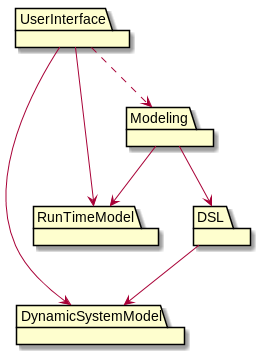
\includegraphics[width=0.5\linewidth]{package-diagram}
\caption{Общая структура программного комплекса.\\Обычные стрелки --- явные зависимости.\\Пунктирные --- неявные.}
\label{fig:package-diagram}
\end{figure}
\FloatBarrier
Таким образом можно выделить следующие библиотеки в программном комплексе (рис. \ref{fig:package-diagram}):
\begin{itemize}
	\item DynamicSystemModel~--- модель данных динамической системы. Содержит типы данных, описывающие структуру вычислительной сети.
	\item DSL~--- предметно-ориентированный язык и инструменты работы с языком, необходимые для преобразования в модель данных.
	\item RunTimeModel~--- модель данных процесса моделирования. Содержит типы данных, необходимые для обмена информацией и исполнении команд модуля визуализации и управляющей программы.
	\item Modeling~--- управляющая программа, производящая моделирование и сбор данных об исполнении программы.
	\item UserInterface~--- модуль визуализации. 
	На схеме представлен, как один компонент, однако может быть представлен группой схожих компонент, построенных на основе пакетов с моделями данных. 
	Ввиду того, что Kotlin позволяет создавать мультиплатформенные программы, описанные в пакетах моделей данных классы могут быть преобразованы скомпилированы и использоваться в различных языках. 
	Это позволит иметь единую базу исходных кодов для реализаций клиентского приложения для различных платформ: браузеров, оконных приложений на Java или Kotlin, оконных приложений на C++, интерфейс командной строки, а также для интеграции с другим ПО.
\end{itemize}

Такая архитектура обособляет данные и способы взаимодействия с ними, что позволяет отделить различные части приложения и обеспечить максимально низкую их зависимость друг от друга.
При подобном разбиении так же облегчена задача обмена данными между сообщающимися модулями, т.к. они используют единый способ представления данных.


